\providecommand{\main}{../../..}
\documentclass[\main/main.tex]{subfiles}
\begin{document}

\subsection{Esercizio 3}
Si descriva brevemente il metodo della trasformazione inversa per enumerare le soluzioni paretiane, specificandone le condizioni di applicazione.

Si applichi tale metodo al seguente problema:

\begin{align*}
	\max f_1  = x_1 + x_2  \\
	\max f_2  = x_1 - x_2  \\
	x_1^2 + x_2^2 & \leq 1 \\
	x_1 \leq 0
\end{align*}

\subsection{Soluzione esercizio 3}

\subsubsection*{Metodo della trasformazione inversa}
Si determina l'inversa della funzione $f$, $\phi: F \rightarrow X$, si sostituisce $x = \phi(x)$ nei vincoli e quindi si ottiene il sottoinsieme $F^o$ degli impatti preferibili e da quest'ultimo si ottiene quindi la regione paretiana $X^o$. È applicabile solo quando $f \in \mathbb{R}^2$.

\subsubsection*{Determino l'inversa $\phi$}
\[
	\begin{cases}
		f_1  = x_1 + x_2 \\
		f_2  = x_1 - x_2
	\end{cases}
	\Rightarrow
	\begin{cases}
		f_1  = 2x_1 - f_2 \\
		x_2  = x_1 - f_2
	\end{cases}
	\Rightarrow
	\begin{cases}
		x_1  = \frac{f_1 + f_2}{2} \\
		x_2  = \frac{f_1 - f_2}{2}
	\end{cases}
\]

\subsubsection*{Sostituisco l'inversa nei vincoli}
\[
	\begin{cases}
		\left( \frac{f_1 + f_2}{2} \right)^2 + \left(\frac{f_1 - f_2}{2}\right)^2 \leq 1 \\
		\frac{f_1 + f_2}{2} \leq 0
	\end{cases}
	\Rightarrow
	\begin{cases}
		\left( f_1 + f_2 \right)^2 + \left(f_1 - f_2\right)^2 \leq 4 \\
		f_1 + f_2 \leq 0
	\end{cases}
\]

L'immagine della regione paretiana $F^o$ è l'insieme di punti che non ammettono altri punti nel quadrante in basso a sinistra, che in questo caso costituiscono il segmento evidenziato in rosso nella figura \ref{area_paretiana_3}.

\begin{figure}
	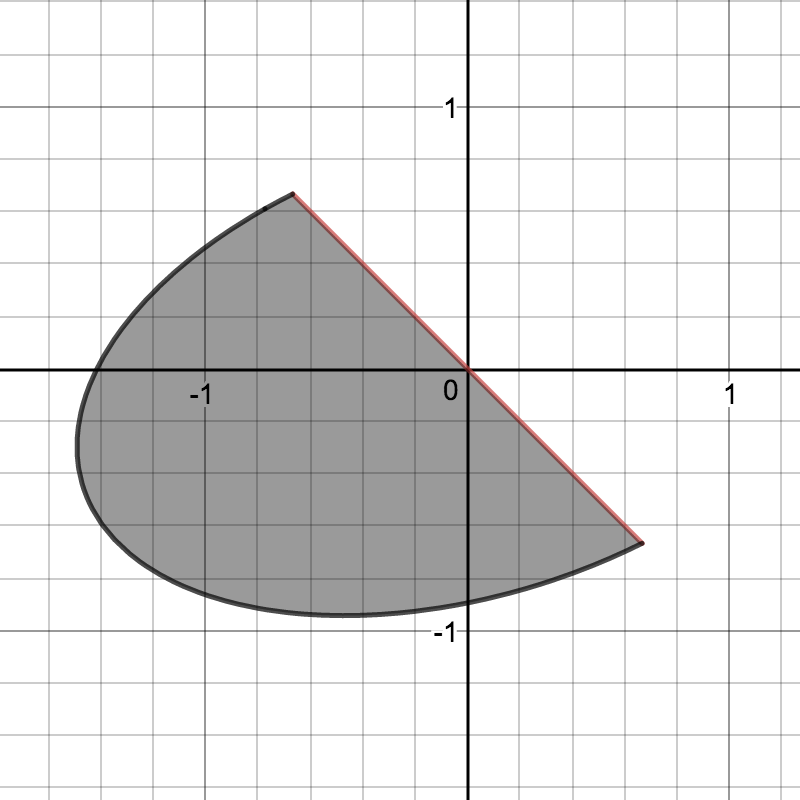
\includegraphics[width=0.3\textwidth]{14362016}
	\caption{In rosso l'immagine della regione paretiana.}
	\label{area_paretiana_3}
\end{figure}

La trasformazione inversa in questo caso è \textbf{lineare}, quindi anche la regione $X^o$ risulterà un segmento di retta.

I due punti risultano essere: $A = (-1, 1)$ e $B = (1,-1)$.

Calcolo quindi i punti che determina il segmento della regione paretiana.

\[
	\begin{cases}
		x_1  = 0 \\
		x_2  = \pm1
	\end{cases}
\]

Da cui i due punti che determinano il segmento della regione paretiana $X^o$ sono $C = (0, -1)$ e $D = (0, 1)$.

\begin{figure}
	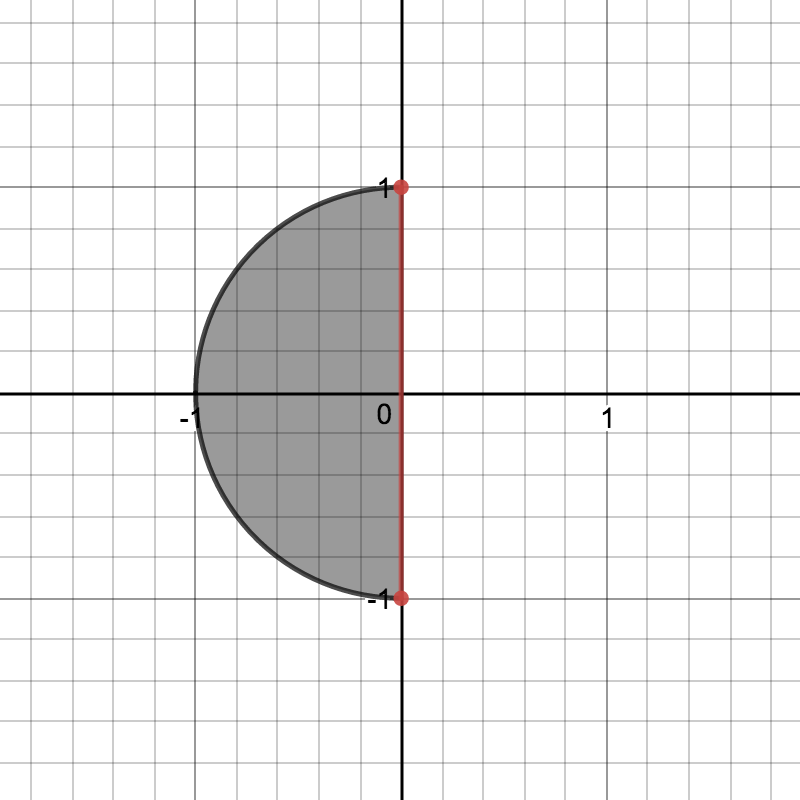
\includegraphics[width=0.3\textwidth]{14362016X}
	\caption{In rosso la regione paretiana.}
	\label{area_paretiana_4}
\end{figure}

\end{document}